\documentclass[a4paper,titlepage,12pt]{book}
\usepackage[suftesi]{frontespizio}
\usepackage{geometry}
\usepackage{lmodern}
\usepackage[italian]{babel}
\usepackage[dvipsnames]{xcolor}
\usepackage{imakeidx}[column=1, title=Indice, intoc]
\usepackage{subfig}
\usepackage{graphicx}
\definecolor{blu_pant}{RGB}{0, 64, 122}
\geometry{margin=1.2in}
\makeindex[columns=1, title=Indice, intoc]
\begin{document}

\begin{frontespizio}
\Logo{images/Universita-pisa.jpg}
\Istituzione{Università di Pisa}
\Dipartimento{Informatica}
\Corso[Laurea Triennale]{Informatica \\(classe L-31)}
\Annoaccademico{2021--2022}
\Titoletto{Relazione di Tirocinio presso l'azienda Zerynth S.R.L.}
\Titolo{\textcolor{black}{Integrazione di una piattaforma \\di veichle tracking esistente \\con l'architettura cloud di Zerynth}}
\Sottotitolo{}
\Candidato[578138]{Andrea Tufo}
\NRelatore{Tutore Aziendale}{}
\Relatore{Davide Neri}
\NCorrelatore{Tutore Accademico}{}
\Correlatore{Gabriele Mencagli}
\end{frontespizio}

\tableofcontents


\sffamily
\chapter{
\sffamily
Introduzione\index{Introduzione}}
Questo progetto aveva come scopo principale quello di integrare un sistema già esistente per il tracciamento veicolare, ovvero Traccar, con la piattaforma zCloud sviluppata dall'azienda Zerynth s.r.l.\\
zCloud, è a tutti gli effetti una piattaforma cloud che permette agli utenti registrati all'interno del servizio, di aggiungere device, fleet e workspace. Il device rappresenta il digital twin di un device fisico, esso possiede degli attributi, tra i principali abbiamo un identificatore, un nome, un id dell'account a cui appartiene e un id relativo al fleet in cui è contenuto. Il fleet invece è un insieme di dispositivi registrati, e anch'esso possiede un id ed un nome. Infine abbiamo le workspace, ovvero, degli spazi di lavoro in cui l'utente può decidere di aggiungere fleet e device.\\
Traccar invece, è un sistema di tracciamento di dispositivi, possiede un'interfaccia grafica dove è possibile osservare il movimento real-time del dispositivo, i suoi attributi, dei report generati e customizzabili e anche delle geofence ovvero delle aree limitate che l'utente può decidere di disporre sulla mappa. Il sistema permette inoltre di ricevere delle notifiche per qualsiasi evento l'utente decida di registrarsi, come ad esempio entrata in una geofence (o uscita dalla geofence), dispositivo che iniza a muoversi o che si ferma o batteria del device bassa. Anche Traccar possiede le proprie entità come ad esempio i device, i gruppi, ma a differenza di zCloud non possiede il concetto di workspace.\\
Uno dei primi problemi che ho dovuto affrontare è stato sicuramente comprendere tramite la documentazione e tramite alcun simulazioni effettuate in ambiente docker, il funzionamento di Traccar, delle API fornite delle funzionalità offerte dal servizio. Successivamente ho dovuto confrontare mettere a confronto le due piattaforme e cercare di analizzare differenze e similitudini, specialmente per quanto riguarda gli oggetti trattati. Il secondo problema, non più di tanto complesso, era provare a trovare una mappatura del concetto di workspace in Traccar,  e la soluzione adottata è stata quella di rappresentare uno spazio di lavoro come un gruppo di Traccar che non avesse parenti. \\
Dopo aver realizzato personas, use-cases e requirements, il passo seguente è stato quello di integrare Traccar con i servizi di zCloud in locale, sempre sfruttando docker e docker-compose. Qui ho incontrato notevoli difficoltà, sia per comprendere come funzionassero i servizi di zCloud e quindi comprendere affondo i vari docker-compose dei servizi e anche tutta la struttura del server Nginx con i relativi file di configurazione, sia per quanto riguarda Traccar stesso, che dopo alcuni aggiornamenti da parte dei mantainers si è dimostrato instabile. Una volta integrato il sistema di Traccar con l'interfaccia web all'interno del server nginx che gestisce tutti i servizi di zerynth, ho dovuto modificare in molti punti il codice sorgente di Traccar. Le modifiche apportate erano essenzialmente mirate all'integrazione effettiva, e quindi permettere l'accesso degli utenti, già registrati in zCloud, all'interno del servizio di veichle tracking senza dover costringere loro di dover effettuare nuovamente un login, tutto quello che concerne l'inizializzazione degli elementi che l'utente possiede e infine anche la comunicazione con i device. Soprattutto la prima parte, ovvero quella relativa all'accesso, è stata particolarmente impegnativa, in quanto Traccar non permette di accedere tramite terze parti, e quindi sono stato costretto a modificare intere parti di codice, sia lato server che lato client. Anche per quanto riguarda i device......


\sffamily
\chapter{
\sffamily
Background e strumenti utilizzati}
Le conoscenze che ho acquisito durante il corso di studi mi hanno aiutato a comprendere le basi di partenza del lavoro che sarei andato a svolgere durante il tirocinio. Pur premettendo che buona parte degli argomenti erano quasi del tutto nuovi per me, come ad esempio la configurazione di un server nginx o l'utilizzo dei microservizi all'interno di una architettura cloud già esistente o l'utilizzo di docker e docker-compose, non ho avute grossissime difficoltà nell'apprendere tutto ciò che mi era nuovo.


\sffamily{
\section{\sffamily
API REST}
L'utilizzo delle API è stato fondamentale per lo svolgimento del progetto di tirocinio. Le API (application programming interface) REST (Representational State Transfer) sono molto diffuse nel mondo della programmazione web e nella realizzazione di protocolli client server. Il sistema REST è infatti basato su HTTP e quindi si basa sulla tipologia di comunicazione client-server. L'architettura REST infatti è basata su chiamate HTTP e prevede una struttura delle url ben definita dal server in quanto ognuna di essa rappresenterà poi una risorsa messa a disposizione dal client. Qui entrano in gioco le API che essenzialmente rappresentano delle funzionalità che il client può chiedere di eseguire da remoto al server, come ad esempio la creazione di un entità o la cancellazione di quest'ultima. Il server quindi espone alcune url rendendole disponibili al client, facendo in modo che chiamando quelle specifiche url, con dei valori di parametri specificati e il payload corretto, il server possa svolgere una determinata funzionalità.....RISCRIVI MEGLIO.\\
Il formato per il trasferimento di file nelle chiamate api è il formato Json, che è un linguaggio di formattazione. La sua diffusione a discapito del formato xml, è dovuta sia alla notevole integrabilità con il linguaggio javascript, presente quasi ovunque nelle pagine web, sia per una verbosità decisamente minore.\\
Questa tecnologia strutturale è davvero molto diffusa in quanto nonostante richieda un leggero effort da parte del client che deve effettuare delle chiamate http strutturate in maniera adeguata ogni qual volta desideri sfruttare una funzionalità del server, comunque rimane un approccio flessibile, scalabile e molto semplice da implementare.
}




\sffamily
\section{\sffamily
Docker e docker-compose}
Il primo strumento utilizzato è una piattaforma che permette di eseguire in un ambiente sicuro applicazioni tramite codice sorgente o immagini, ovvero Docker. Docker infatti da la possibilità di creare un \textit{container}, ovvero un contenitore nel quale è possibile eseguire uno script o più in generale del codice. Ma la vera caratteristica utile di docker, è docker-compose, ovvero la possibilità di collegare più applicazioni e quindi più container tra di loro in una network. A tutti gli effetti viene realizzata una vera e propria rete docker, in cui le applicazioni che sono in esecuzione su essa possono comunicare tra loro scambiandosi dati e informazioni.\\
Ogni servizio di una rete di docker-compose ha essenzialmente due file principali: il docker-compose.yml ed il Dockerfile. Il primo è in pratica un insieme di regole che quel servizio deve seguire prima di avviare la propria esecuzione o durante la propria esecuzione, come ad esempio le porte che deve esporre, l'hostname all'interno della rete docker o anche le dipendenze che ha nei confronti degli altri servizi. Il Dockerfile presente anche in docker, è paragonabile ad un makefile, ovvero una sequenza di comandi che il sottosistema con kernel linux simulato deve eseguire.\\
Docker infatti è a tutti gli effetti un sistema virtuale, e come tale è implementata una simulazione di un kernel Linux, sulla quale vengono eseguiti in modo del tutto isolato i diversi container.
Per far questo docker isola a livello di sistema i conteiner limitando risorse come per esempio la CPU o quantità di memoria usufruibile da un container, rendendo così ogni servizio indipendente dagli altri a livello di risorse utilizzate. Docker riesce a far ciò utilizzando librerie per interfacciarsi con il sistema linux ed utilizzare funzionalità come namespace che offre la possibilità di limitare ciò che un processore o un insieme di processori può vedere a livello di informazioni relative, ad esempio, agli utenti come il loro Id, e cgroup che permette di associare ad un gruppo di processi delle limitazioni di risorse hardware (quantità di CPU, memoria, rete) e software (permessi alle risorse).

\sffamily
\subsection{\sffamily
Utilizzo di docker e docker-compose}
Questi due strumenti li ho entrambi utilizzati in primis nella simulazione che ho effettuato per studiare il sistema ed il funzionamento di Traccar e delle sue API e successivamente per testare l'integrazione di Traccar con i microservizi di zcloud all'interno della architettura cloud in locale. \\
All'interno dell'architettura erano presenti alcuni servizi come "portainer" che permette di visualizzare graficamente i container, i logs di ogni container, ed è stato un utilissimo strumento di debug. Oltre a portainer, è possibile citare tra i servizi principali che presentano un ambiente grafico, "pgadmin" per monitorare il database in postgres e "rqm" che permette di visualizzare lo stato delle code rabbitMQ.

\sffamily
\section{\sffamily
Code rabbitMQ}
Durante la fase centrale del progetto ho dovuto affrontare la parte relativa alla gestione dei dati inviati dai device tracciabili a Traccar. Dunque ho dovuto gestire questi ultimi inviandoli a code rabbitMQ presenti su zcloud che avrebbero poi svolto il compito di fare lo storage dei dati sul database di zcloud.\\
Le code rabbitMQ non sono altro che un ausilio per realizzare la struttura publish-broker-subscribe del protocollo mqtt. Infatti ogni coda rabbitMQ rappresenta un topic sul quale i device pubblicano, o meglio, ogni coda possiede una "binding-key" (o routing-key) ovvero una chiave univoca la che identifica.
In realtà il funzionamento delle librerie di rabbitMQ è leggermente diverso ed un po' più complesso.\\
Partiamo col dire che una coda rabbitMQ possiede come entità un \textit{publisher} che pubblica i dati su una coda, ed un \textit{consumer} che prende i dati dalla coda a cui è inscritto. Inoltre è presente un'ulteriore entità, l'\textit{exchange}, che rappresenta un intermediario tra il publisher e la coda. L'exchange ha il compito di scegliere come e dove pubblicare il dato ricevuto dal publisher secondo un algoritmo specifico. Le tipologie di algoritmi principali sono quattro: fanout che invia dati a tutte le code presenti, direct che inoltra il dato solo alla coda alla quale viene indicato il topic del publisher, e poi abbiamo header e topic. Nel mio caso la tipologia era quella di un exchange topic, ovvero molto simile alla tipologia direct ma con la differenza che in questo caso le routing-key non hanno una qualsiasi struttura, bensì sono costruite in un modo specifico. Una routing-key in questo caso quindi è a tutti gli effetti una lista di parole delimitate da punti come ad esempio \textit{j.data.dev-87y.temp}.
E' bene specificare che mentre il publisher ed il subscribe rappresentano delle entità che devono essere implementate, l'exchange è un oggetto che già esiste, è necessaria esclusivamente la sua configurazione.\\
Nel mio caso specifico ho utilizzato le librerie di java per rabbitMQ, ed una volta individuato il punto del codice sorgente di Traccar in cui viene gestita la comunicazione con i device, ho implementato un publisher che pubblica i dati che aveva ricevuto dal device su una coda rabbitMQ presente sul cloud di zerynth.\\
L'exchange iin zCloud era nominato \textit{amq.topic}, mentre la binding key era nominata \textit{data}. L'intero sistema di gestione delle publish dei device è stato gestito in modo tale che i device comunicassero direttamente a traccar, in cui tramite l'aggiunta di un apposito handler, dopo aver eseguito l'autenticazione e l'autorizzazione del dispositivo sfruttando microservizi interni allo zCloud, viene invocata l'esecuzione di un metodo presente all'interno di una classe, realizzata per gestire le interazioni con i vari servizi di zCloud, detto \textit{publishOnRMQ} in cui viene effettuata la scrittura sulla coda precedentemente indicata con il tag \textit{latlon}, che indica un dato relativo alla posizione del device. Infatti viene memorizzato un vero e proprio file json che corrisponde al marshalling di un entità detta \textit{position} presente in Traccar.
\chapter{
\sffamily Studio del sistema e analisi dei requisiti}

La prima parte del tirocinio era composta da due fasi, ovvero uno studio preliminare della piattaforma, comprendere quali erano le entità coinvolte, come erano fatti gli oggetti che Traccar creava e gestiva (user, device, gruppi) e soprattutto uno studio mirato alle API fornite da Traccar stesso; la seconda fase invece è consistita nel trovare un parallelismo tra le entità di Traccar e le entità di zCloud, discutendone analogie, differenze e similitudini, e successivamente pensare a come si sarebbe potuto costruire il workflow di un utente generico che intendesse aggiungere su zCloud un device tracciabile, definendo quindi personas, user stories, use cases e requirements.\\

\section{
\sffamily Studio della piattaforma Traccar}
Per comprendere al meglio le funzionalità che Traccar offriva, dopo aver analizzato la documentazione, ho realizzato una simulazione utilizzando docker e docker-compose.\\
La simulazione consisteva in un server costituito da una immagine di Traccar, un database postgres, e un client scritto in go che utilizzasse la maggior parte delle api fornite da Traccar. Il client infatti aveva una fase di inizializzazione in cui eliminava tutti gli oggetti creati da un'esecuzione precedente dal server nel caso in cui questi oggetti fossero presenti, altrimenti procedeva con l'inizializzazione dell'ambiente e quindi con la creazione dei devices dei groups e delle altre entità che Traccar offre.\\
Da questo studio delle API di Traccar sono emerse tutti i punti di forza e tutte le criticità di Traccar, e qui di seguito proverò a riassumerle in modo da capire meglio quali sono le problematiche che io ed il mio tutore aziendale abbiamo dovuto affrontare durante il corso del tirocinio.\\


\subsection{
\sffamily Come funziona Traccar}
La piattaforma da integrare ha essenzialmente la tipica struttura di una web application, costituita da un server, più precisamente un Jetty Web Server, che espone delle API e le websocket, un client e un database. Il server si occupa di gestire tutte le richieste dei vari client che interagiscono con esso tramite web app, mentre le connessioni con i devices sono gestiste da una Netty network pipeline che comunica indirettamente con il web server. \\
Questa piattaforma supporta molteplici tipi di protocolli per quanto riguarda i device e nel caso ad esempio ndlla mia simulazione ho utilizzato il protocollo OSMand (OpenStreetMap Automated Navigation Directions) poiché è davvero semplice da rispettare ed applicare. I device infatti pubblicano la loro posizione e i loro attributi direttamente al server utilizzando il protocollo scelto, compreso il loro uniqueId tramite il quale il sistema riesce ad identificare univocamente il device fisico associato al suo digital twin. Il database di default di Traccar è utilizzabile solo per quanto riguarda la fase di testing, mentre è consigliabile, da quanto riportato dalla documentazione di tracccar di utilizzare un database esterno per la fase di sviluppo. 

\begin{center}
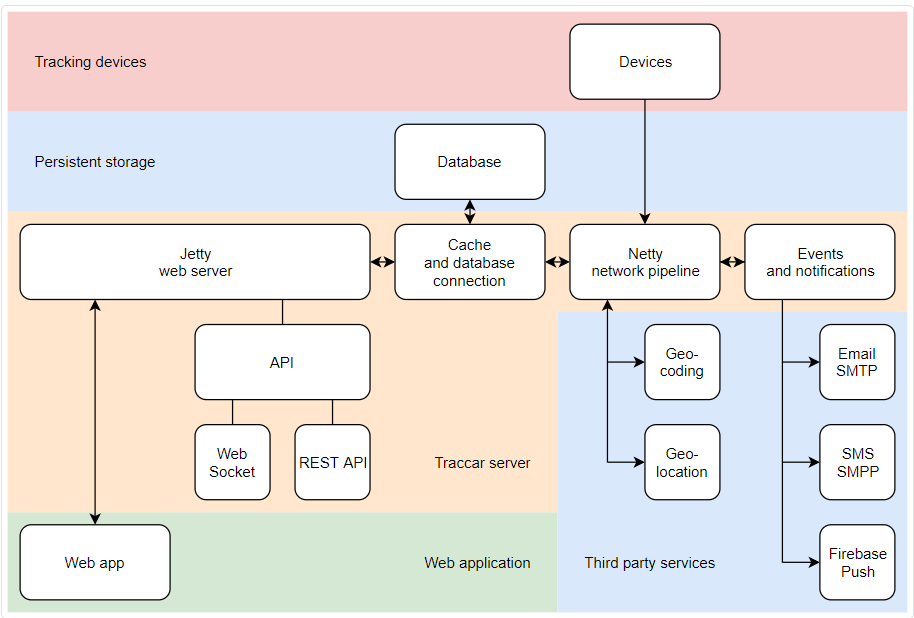
\includegraphics[scale=0.7]{images/arcTraccar.png} \\
\textit{Figura 3.1.1: Architettura di traccar}\label{fig:}
\end{center}


\subsection{
\sffamily Architettura di ZDM}
L'architettura del cloud di Zerynth è composta da tanti microservizi che cooperano per svolgere azioni e funzionalità specifiche. Nel mio caso ho dovuto spesse volte interfacciarmi con molti di questi microservizi per poter accedere ad esempio ai database di zerynth sia in scrittura che in lettura. \\
Giusto per citarne alcuni: \textit{rpgboucer}, \textit{login-service}, \textit{wfd-service}, \textit{dev-authorization-service}, \textit{dev-authentication-service}. Il primo permette di accedere solo in lettura ad un particolare database di Zerynth chiamato \textit{zStorage}\footnote{\sffamily I database in zerynth sono principalmente tre zCloud, ZDM e zStorage, nell'ultimo in particolare vengono memorizzati per ogni workspace tutti i dati pubblicati dai device} composto a sua volta da sei partizioni, tre dette "master" e tre "repliche" dei relativi master.\\
Il servizio di login-service permette di autorizzare un utente registrato, e nel mio caso ho utilizzato questo servizio indirettamente, e più avanti nel documento verrà spiegato meglio nel dettaglio.\\
In seguito abbiamo il wfd-service che in realtà ho dovuto modificare, in quanto questo servizio gestisce la creazione, l'aggiornamento e la rimozioni delle entità all'interno dello zCloud, ed infine i servizi dev-autentication e dev-authorization, indispensabili per l'autenticazione del device e per autorizzare quest'ultimo ad utilizzare le risorse all'interno dell'architettura di zerynth.

\subsection{
\sffamily Caratteristiche di Traccar}
Traccar offre una caratterizzazione del proprio spazio di lavoro (anche se come vedremo dopo non esiste in realtà il concetto di "workspace" di un utente), infatti si ha la possibilità di aggiungere una "geofence" per limitare un'area specifica che può essere realizzata con qualsiasi tipo di forma, delle "notifications" per ricevere delle notifiche sugli eventi a cui si è interessati, aggiungere dei "commands" ovvero degli attributi calcolati sulla base degli attributi base che un device possiede. Inoltre un'altra cosa di rilievo è senza dubbio poter personalizzare ogni singolo device aggiungendo un set potenzialmente infinito di attributi custom. Da segnalare anche la possibilità di poter usufruire dei reports personalizzabili e anche di grafici riguardanti i device associati ad un profilo. \\

\subsection{
\sffamily Problematiche emerse}
Purtroppo sono emerse diverse problematiche durante il corso del progetto e molte scelte effettuate in fase di analisi sono state modificate in quanto nelle fasi più mature del progetto è migliorata la consapevolezza degli strumenti e la conoscenza del codice stesso di traccar. \\
Una delle problematiche più importanti è certamente la mancanza di accedere al servizio da terze parti utilizzando dei token d'accesso. O meglio, è possibile estendere le funzionalità di traccar per l'autenticazione in modo tale da sfruttare il protocollo LDAP per l'autenticazione da terze parti. Nonostante ciò questa ipotesi è stata scartata in quanto poco pratica da realizzare e quindi la strada presa è stata quella di estendere direttamente il codice sorgente di traccar.\\
Inoltre anche il claiming del dispositivo è stato un passo importante da realizzare in quanto traccar non supporta l'utilizzo di token firmati da parte dei device, bensì l'autenticazione dello stesso è effettuata solo tramite l'analisi del codice IMEI del device.

\section{
\sffamily Struttura di zCloud}
zCloud ha un'impostazione leggermente diversa da Traccar, in quanto permette di creare per ogni utente diversi spazi di lavoro, ma nonostante ciò alcuni oggetti sono molto similari. In zCloud ogni utente ha la possibilità di creare da una a più workspace, in ogni workspace da zero a più fleet e in ogni fleet da zero a più device. Analizzeremo adesso la struttura dei json di ogni elemento di zCloud, confrontandola con quella dell'oggetto che ho deciso di mappare in Traccar.


\section{
\sffamily Parallelismo Traccar e zCloud}
In questa fase era necessario trovare una soluzione ai problemi che erano sorti con questa fase di studio preliminare di Traccar. Come prima cosa bisognava trovare una relazione tra le varie entità e quindi capire come codificare un oggetto presente in zCloud in uno di Traccar nel modo migliore possibile. Come vedremo qui di seguito il problema più grande sarà rappresentato dalla workspace, entità che in zCloud esiste ma che in Traccar no.



\paragraph{
\sffamily Device}
Il device in zCloud ha una forte similarità con il device in Traccar, qui di seguito presento il json dell'oggetto di Traccar a quello di zCloud.\\



\begin{center}

\begin{tabular}{c c c c}

    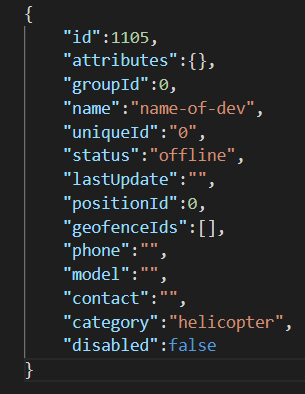
\includegraphics[scale=0.8]{images/traccDev.png}

    \label{fig:my_label}

 &  
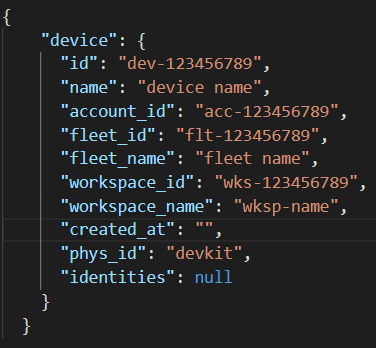
\includegraphics[scale=0.6]{images/zClDev.png} \\
\textit{JSON del device in Traccar} &  \textit{JSON del device in zCloud}
\end{tabular}
\end{center}\par\medskip


Abbiamo infatti una corrispondenza quasi uno a uno con molti attributi, quali ad esempio \textit{id}, \textit{name}, che sono ovvie ed intuitive. Inoltre anche attributi come il \textit{fleet\_id}, il \textit{workspace\_id} ed il \textit{pyhs\_id} in zCloud hanno una corrispondenza implicita ma che comunque esiste. Tratterò l'argomento della workspace in seguito,  perciò adesso mi concentrerò sul \textit{fleet\_id} e sul \textit{phys\_id}. Il primo può essere perfettamente mappato con il \textit{group\_id}, poiché come vedremo successivamente, il fleet è simile al group di Traccar,il \textit{pys\_id} invece è in relazione con lo \textit{uniqueId} essendo entrambi due identificatori univoci del dispositivo fisico. Infine \textit{account\_id} in zCloud può essere in realtà ignorato dato che ogni dispositivo in Traccar è collegato al suo user, in quanto osservando lo schema relazionale, esiste un collegamento tra la tabella degli user e quella dei device.\\
Per i restanti attributi, nel caso in cui dovessero essere necessar, si può ricorrere alla creazione di nuovi attributi nell'entità di Traccar, utilizzando il tag \textit{attributes}.

\paragraph{
\sffamily Fleet}
Per quanto riguarda i fleet, come già accennato in precedenza, ho trovato una relazione con il group di Traccar, qui di seguito il confronto con i due JSON degli oggetti.




\begin{center}

\begin{tabular}{c c c c}

    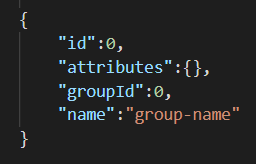
\includegraphics[scale=0.8]{images/traccGr.png}

    \label{fig:my_label}

 &  
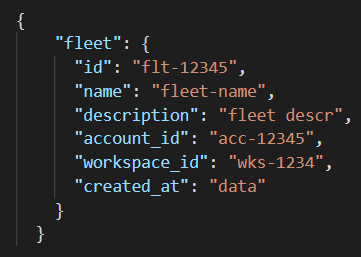
\includegraphics[scale=0.7]{images/zClGr.png} \\
\textit{JSON del group in Traccar} &  \textit{JSON del fleet in zCloud}
\end{tabular}
\end{center}\par\medskip


Vale anche qui il discorso fatto per i device, si vede molto chiaramente come le due entità sono molto simili. E' importante evidenziare come in traccar ci sia anche un \textit{groupId} da non confondere con l'\textit{id}, in quanto il primo indica l'indic del gruppo parent a cui appartiene, infatti in Traccar un gruppo può avere infiniti sottogruppi a cui fa da parent. 

\paragraph{
\sffamily Workspace}
Terminando l'analisi con la workspace, dopo aver pensato a diverse idee su come modellarla in Traccar, la soluzione che ho preso è stata quella di mapparla come un group che non ha parent. Una workspace quindi è a tutti gli effetti un gruppo che ha l'\textit{groupId} sempre a zero, in quanto non appartiene a nessun gruppo. Tutti i suoi gruppi figli invece, faranno essenzialmente le veci dei fleet.\\
Grazie a questa caratteristica di Traccar, ovvero che l'entità del group è qualcosa di generico, che rappresenta un inseme di elementi eterogenei, è stato possibile mappare con successo anche la workspace di zCloud, ecco qui di seguito una rappresentazione grafica della mappatura workspace e group.


\section*{}
\begin{center}
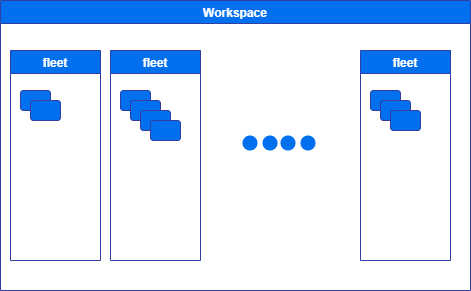
\includegraphics[scale=0.6]{images/zc_ws.png}\\ 
\textit{Workspace di zCloud}\\
\section*{}
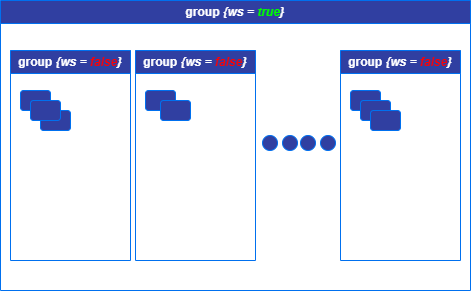
\includegraphics[scale=0.6]{images/traccar_ws.png} \\
\textit{Workspace mappata in group in Traccar}


\end{center}

\section{
\sffamily Personas e requisiti}
l'Ultimo passo prima di iniziare l'implementazione e l'integrazione effettiva del servizio traccar, è stato quello di descrivere alcuni archetipi di potenziali utilizzatori del servizio e quindi successivamente definire i possibili requirements.\\
in questa fase ho analizzato tre personas di cui due di queste appartenenti al mercato B to B e una sola personas che svolgeva il ruolo di consumer normale. Le aziende che potrebbero voler usufruire di questo servizio possono quindi essere legate al mondo dei trasporti, all'ambito militare o nel noleggio di veicoli come ad esempio tutte quelle realtà che si occupano di micromobilità.\\
Prima di passare ai requisiti ho realizzato alcuni use cases, azioni che l'utente potrebbe potenzialmente svolgere sul sistema in sviluppo. Prendendo ad esempio la creazione di un device tracciabile, ecco qui di seguito lo schema del suo caso d'uso:\\
CASO DUSO\\
E quindi sono infine passato ai requisiti tra i quali abbiamo ad esempio:
\begin{itemize}
\item L'utente non può aggiungere lo stesso device tracciabile due volte;
\item Una workspace abilitata a tracciabile può contenere solo device tracciabili;
\item Una workspace non abilitata a tracciabile non può avere device tracciabili;
\item L'utente può avere lo stesso device su due o più workspace.\\
\end{itemize}

\sffamily
\chapter{
\sffamily Integrazione del sistema}
Per integrare correttamente il sistema di Traccar con la piattaforma di zerynth, è stato necessario mettere in collegamento il servizio di tracciamento dei dispositivi con i microservizi interni dell'architettura cloud di zCloud. E' stato dunque fondamentale capire come realizzare le chiamate api agli entrypoint che i servizi di Zerynth esponevano e codificare i dati ottenuti da essi per poi poterli utilizzare correttamente. \\
La fase iniziale dell'intero processo di implementazione è consistita nell'inserire traccar all'interno dei servizi di zCloud, connettendo il servizio all'intera architettura. Per far ciò ho dovuto implementare un flie di configurazione di traccar e inserirlo nell'apposita directory, nella quale era situata tutta la configurazione di Ngnix. Successivamente è stato necessario autenticare l'utente attraverso l'account id che il \textit{login-service} di zCloud inviava come response nel caso in cui una autenticazione di uno user fosse andata a buon fine, e poi passare anche all'autenticazione e autorizzazione dei device che avrebbero dovuto poi comunicare con traccar. \\
Ovviamente per poter testare (ovviamente inizialmente tutto in locale) le singole fasi di implementazione, era necessario avvalersi di una simulazione di un device che invia dati al servizio traccar. Per far ciò ho realizzato un piccolo script in golang che invia dati al sistema utilizzando il protocollo OsmAnd \footnote{\sffamily OsmAnd (OpenStreetmap Automated Navigation Direction protocol) è un protocollo di live tracking utilizzato dall'omonimo software di tracciamento OsmAnd, esso si può realizzare, lato device, inserendo nella url, alla quale il dispositivo intende mandare i dati, tutti i parametri necessari alla localizzazione e identificazione del device stess. Un esempio di url strutturata in base al protocollo OsmAnd è il seguente: "http://tracking.org:5023/?id=23\&lat=34.4\&lon=2.4\&speed=0\&alt=2345"}(scelta esclusivamente per una questione di praticità, il protocollo OsmAnd è molto semplice da realizzare) emulando quindi gli spostamenti di un dispositivo che si muove sulla mappa.

\section{\sffamily
Configurazione di Traccar in NGNIX}
In questa parta ho realizzato il primo collegamento con traccar e la struttura di zCloud, collegando il servizio al proxy server. Oltre a specificare il dominio con il quale Traccar sarebbe diventato raggiungibile dagli host esterni all'architettura di zCloud, la connessione ad NGNIX permette alla piattaforma di delegare le operazioni di default al cloud e quindi ai microservizi interni. Ad esempio, una delle principali azioni che in parte viene delegata ad uno dei servizi di Zerynth è l'autenticazione dello user quando intende accedere a traccar. \\
NGNIX infatti inoltra la richiesta di login da parte di un utente ad un servizio chiamato \textit{login-service}, il quale si occupa di verificare l'esistenza di tale utente, e nel caso in cui l'autenticazione andasse a buon fine login-service restituisce un parametro al proxy-server, ovvero l'account id dell'utente appena verificato. NGNIX dunque inserisce questo identificativo all'interno di un campo dell'header, così da poter permettere a tutti i servizi interni di identificare l'autore delle richieste interne che si scatenano in cascata.\\
Qui di seguito una piccola rappresentazione grafica della connessione di traccar all'architettura cloud di Zerynth.\\

\begin{center}
\centering
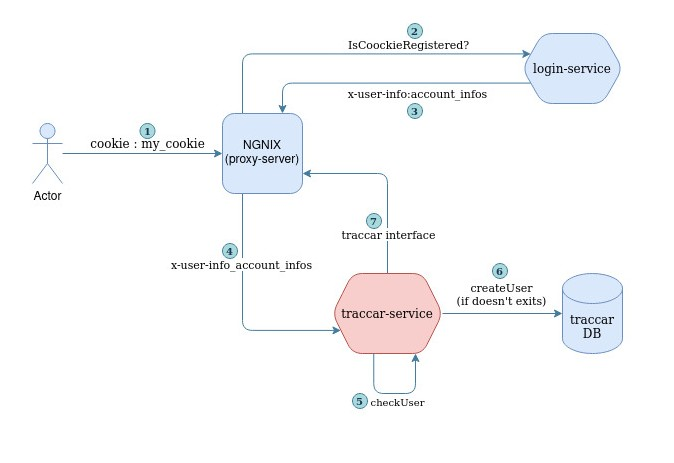
\includegraphics[scale=0.6]{images/traccar_login_serv.jpg}\\ 
\textit{Figura 4.1: Prima fase di integrazione di traccar}\label{fig:}

\end{center}

Per completare la configurazione di traccar con NGNIX era fondamentale inserire anche l'inoltro delle connessioni per le web-socket, in quanto i client si connettono ad esse per aggiornare i dati riguardanti i device e in generale le entità presenti. Qui di seguito ecco illustrato nel dettagliko il file di configurazione per NGNIX di traccar.\\
IMMAGINE TRACCAR:CONF\\

\section{\sffamily
Autenticazione dell'utente in Traccar}
Il normale funzionamento di traccar prevede un login composto da username e password per accedere al servizio. Ma questa soluzione non era naturalmente adeguata al nostro scopo, era infatti necessario poter far accedere l'utente automaticamente una volta che si fosse registrato e avesse effettuato l'accesso su zCloud. In realtà buona parte di questa funzionalità è già realizzata in quanto il cloud possiede un servizio che autentica lo user, citato in precedenza il \textit{login-service}. Questa piccola parte architetturale funziona nel seguente modo, seguendo lo schema in figura 4.1:\\
\begin{enumerate}
\item Il proxy-server NGNIX riceve la richiesta di accesso da parte di un client all'url in cui traccar è specificato come location (ad esempio traccar.zerynth.localhost) con il cookie dell'utente;
\item NGNIX inoltra la richiesta al \textit{login-service} con il cookie che l'utente ha passato nella richiesta precedente;
\item Il servizio restituisce al server NGNIX la response, nella quale cui se l'utente risulta esistere, viene incluso l'account-id di tale utente all'interno di un campo header \textit{x-user-info}.
\item NGNIX inoltra poi la richiesta iniziale, con l'aggiunta del nuovo campo dell'header a traccar.
\end{enumerate}


\subsection{\sffamily
Utilizzo dell'account-id in Traccar}
A questo punto il passo successivo è stato quello di istanziare una nuova sessione di traccar per l'utente. Il client che ha effettuato una richiesta di sessione a traccar dunque è già autenticato dal cloud, quindi non rimase altro che trovare un modo di gestire le informazioni nell'header che NGNIX  inoltra a Traccar, più precisamente l'account-id. Nella classe dove viene gestita la richiesta di una sessione quindi ho dovuto modificare i vari controlli che traccar effettuava, infatti ecco come normalmente era strutturata una richiesta (GET) di sessione all'entrypoint (NOTA ENTRYPOINT) \textit{api/session}:\par\medskip

\begin{center}\begin{flushleft}
HOST: "http://traccar\_url/api/session"\\
HEADER: "Authorization Basic: user\_code64:password\_code64"\par\medskip
\end{flushleft}

\end{center}

Dunque non rimaneva altro che modificare il punto in cui il server elabora la richiesta del client che vuole ottenere una sessione e quindi il punto in cui viene gestito lo scambio di dati all'entrypoint api/session. La classe che si occupa di ciò è \textit{SessionResource.java}, qui ho implementato una logica che ottiene dall'header della richiesta del client l'account-id dell'utente e controlla se è registrato nel db di traccar. Se è vero allora restituisce al client il formato Json con le informazioni relative all'utente, se invece non dovesse esistere nel database di traccar allora viene creata una nuova istanza e restituito il Json con le informazioni sull'utente appena creato, che possiede come nome l'account-id di zCloud.\\
Concludendo posso essere certo quindi, che gli utenti create siano tutti già stati autorizzati dal servizio di login-service e quindi non occore fare aggiuntive verifiche, se non quelle di controllare che l'utente sia già registrato nel database di traccar.

\subsection{\sffamily
Considerazioni sulla soluzione}
Possono essere effettuati dei miglioramenti e delle ottimizzazioni a questa soluzione, però la scelta è stata quella di tenere questa implementazione in quanto essa rappresenta una realizzazione pratica e funzionale, infatti, uno dei problemi che avremmo dovuto affrontare se l'entità utente non fosse salvata nei db di traccar, sarebbe stato quello di mantenere tutti i link con gli oggetti come le geofence e le notification, ovvero tutti quegli oggetti che obbligatoriamente appartengo allo schema relazionale di Traccar. Più avanti vedremo come ho effettuato alcuni tentativi per evitare lo "sdoppiamento" delle risorse e quindi ad esempio avere per uno stesso device un'istanza sul database di traccar e un'altra sul database di zCloud.


\section{\sffamily
Gestione dei device}
La fase immediatamente successiva è stata quella di implementare tutta la fase di gestione dei dispositivi, codificando i dati che inviano a traccar in modo tale da ricavare informazioni da poter utilizzare per chiamare i servizi interni di zCloud. Le decisioni più importanti che sono state prese in questo caso sono state due, ovvero dove dovessero essere salvate le informazioni sulle varie posizioni di un device, e dove dovessero essere memorizzate le informazioni di un device appena creato. \\
Per quanto riguarda la prima parte, la scelta è ricaduta sul salvare le posizioni sullo zStorage di zCloud,in modo tale da permettere anche ad altri servizi all'interno dell'architettura dell'azienda di poter accedere a quei dati, senza dover modificare altri servizi.\\
In generale si può schematizzare tutta la parte relativa ai dispositivi in una sequenza di azioni svolte da traccar, ecco qui di seguito una rappresentazione di questa parte architetturale che comprende solamente la parte di autorizzazione, autenticazione e memorizzazione dei dati.

\begin{center}
\centering
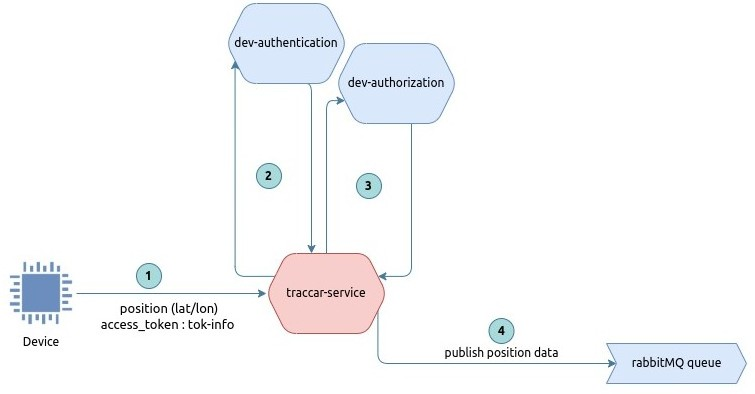
\includegraphics[scale=0.6]{images/dev-aut-traccar.jpg}\\ 
\textit{Figura 4.3: Integrazione dei device tracciabili}

\end{center}







\end{document}